%% Change "letterpaper" in the following line to "a4paper" if you must.

\documentclass[10pt,a4paper]{article}

\usepackage{cogsci}
\usepackage{pslatex}
\usepackage{apacite}
\usepackage{natbib}

\usepackage{color}
\usepackage[fleqn]{amsmath}
\usepackage{amsthm}
\usepackage{amssymb}
\usepackage{stmaryrd}
\usepackage{multicol}
\usepackage{graphicx}

\newcommand{\mvalueof}[1]{\llbracket#1\rrbracket}
\newcommand{\citeposs}[2][]{\citeauthor{#2}'s (\citeyear[#1]{#2})}
\newcommand{\tuple}[1]{\ensuremath{\left\langle #1 \right\rangle}} 

\newcommand{\hl}[1]{\textcolor[rgb]{.8,.33,.0}{#1}}% prints in orange
\newcommand{\hlblue}[1]{\textcolor[rgb]{0.13,0.67,0.8}{#1}}
\newcommand{\argmax}[1]{\underset{#1}{\operatorname{arg}\,\operatorname{max}}\;}
\newcommand{\argmin}[1]{\underset{#1}{\operatorname{arg}\,\operatorname{min}}\;}
\newcommand{\sbna}{\exists\lnot\forall}

\title{Learning biases may prevent lexicalization of pragmatic inferences:\\ a case study combining iterated (Bayesian) learning and functional selection}

\author{{\large \bf Thomas Brochhagen (t.s.brochhagen@uva.nl)} \\
  Institute for Logic, Language and Computation, University of Amsterdam\\
  Science Park, Kruislaan 107, 1098 XG Amsterdam, The Netherlands
  \AND {\large \bf Michael Franke  (mchfranke@gmail.com)} \\
  Department of Linguistics, University of T\"ubingen\\
 Wilhelmstrasse 19, 72074 T\"ubingen, Germany 
    \AND {\large \bf Robert van Rooij (r.a.m.vanRooij@uva.nl)} \\
  Institute for Logic, Language and Computation, University of Amsterdam\\
Science Park, Kruislaan 107, 1098 XG Amsterdam, The Netherlands}


\begin{document}

\maketitle


\begin{abstract}
Natural languages exhibit properties that are difficult to explain from a purely functional perspective. One of these properties is the systematic lack of upper-bounds in the literal meaning of scalar expressions. This investigation addresses the development and selection of such semantics from a space of possible alternatives. To do so we put forward a model that integrates Bayesian learning into the replicator-mutator dynamics commonly used in evolutionary game theory. We argue this synthesis to provide a suitable and general model to analyze the dynamics involved in the use and transmission of language. Our results shed light on the semantics-pragmatics divide and show how a learning bias in tandem with functional pressure may prevent the lexicalization of pragmatic inferences.

\textbf{Keywords:} 
semantics; pragmatics; iterated learning; evolutionary game theory; scalar expressions
\end{abstract}


\section{Introduction}
Why are natural languages structured the way they are and not differently? In particular, what factors are involved in the selection of semantic structure from a space of possible alternatives? A number of recent studies have began to investigate such issues, pertaining to the development and emergence of linguistic features (see \citealt{steels:2015} and \citealt{tamariz+kirby:2016} for recent overviews). While different methodologies have been put forward to this end, the overarching argument is one of competing pressures: natural languages need to enable successful communication, as well as be suited for acquisition. That is, they need to be well-adapted to the communicative needs of their users but they also need to be learnable in order to survive their faithful transmission across generations. 

The present investigation focuses on the interplay of such selective forces by means of a case study on the lexicalization of semantic upper-bounds. Using evolutionary game theory, framed in terms of language use and learning, we investigate the prevalence of a lack of upper-bounds in the literal meaning of scalar expressions. The innovation of the model lies in its combination of functional pressure on successful communication, effects of learning biases on (iterated) Bayesian language learning \citep{griffiths+kalish:2007}, and probabilistic models of language use in populations with distinct lexica \citep{frank+goodman:2012,franke+jaeger:2014,bergen+etal:2015}. Our results show that a learning bias for simple semantic representations coupled with communal language exposure can lead to a prevalence of a lack of semantic upper-bounds provided bounds can be inferred via pragmatic reasoning. This, in turn, offers an explanation to why certain pragmatic inferences fail to lexicalize. 



\section{Conveying and lexicalizing upper-bounds}
A considerably large class of natural language expressions do not lexicalize an upper-bound. That is, they are truth-conditionally compatible with more informative or ``stronger'' alternatives. Here, informativity is understood as an order over entailment. Examples in English include, among many others, numerals such as {\em five} and {\em six}, scalar adjectives like {\em cold} and {\em big}, as well as quantifiers like {\em some} and {\em many}. The commonality of these expressions lies in their literal meaning being compatible with the truth of stronger (relevant) alternatives. For example, if it is true that `Bill read five books' it may well be true that `Bill read six/seven/... books'. Crucially, the latter entails the former; if it is true that `some students came to class' then this would also hold if it were true that `all students came to class'. Prima facie this pattern may seem surprising. If it were true that `some (but not all) students came', then it would putatively serve interlocutors better if {\em some} semantically ruled out the stronger {\em all} case. 

In practice, however, what is communicated often goes beyond the literal meaning of expressions. In particular, mutual reasoning between interlocutors can lead to the enrichment of semantic content \citep{grice:1975}. Such {\em pragmatic reasoning} is driven by interlocutors' mutual expectations of rational language use. In this case the use of a less informative expression when a more informative one could have been used can license a defeasible inference that the stronger alternative does not hold (cf. \citealt{horn:1972,gazdar:1979a}). In this way, a hearer who assumes the speaker to be knowledgeable and cooperative, i.e., able and willing to supply all relevant information at her disposition, can infer {\em some} to be pragmatically strengthened to convey an upper-bounded interpretation. 

This kind of reasoning was already hinted at above: a speaker would have used the more informative alternative if it were true. Since she did not, her addressee can infer that it does not hold. Conversely, a speaker who reasons about her addressee can rely on her drawing this inference. Notwithstanding, while pragmatic reasoning provides an answer to how interlocutors may derive and convey upper-bounds, the question why they are not part of the literal meaning still stands. More generally, while a divide between semantics and pragmatics is commonly agreed upon by linguists, under consideration of purely functional pressures this raises the challenge of providing justifications for the former's structure.

We see two main explanations for a lack of semantic upper-bounds in scalar expressions. The first is that pragmatic reasoning offers a general mechanism to strengthen the meaning of a wide range of expressions when the conditions outlined above hold. Consequently, cases where cooperativity or knowledge are not likely to be given are non-committal to whether stronger alternatives hold. If for all the speaker knows `some students came' but she does not know whether `all came', then the compatibility of {\em some} with (possibly) {\em all} succinctly conveys the speaker's uncertainty about the latter. Given that scalar expressions occur in contexts in which their upper-bounded reading is absent, one could argue for a functional advantage of a lack of semantic upper-bounds: If expressing such a state of affairs is relevant and contextual cues provide enough information for a hearer to discern when a bound is conveyed pragmatically, then doing so is preferred over enforcing the bound overtly through a longer (more complex) expression, e.g. by stating `some but not all' explicitly. That is, all else being equal, speakers prefer to communicate as economically as possible, and pragmatic reasoning enables them to do so. Additionally, this can be contrasted with the hypothetical alternative of lexicalizing two expressions -- one with and one lacking an upper-bound. Four conditions may pressure language to English-like semantics over this alternative: (i) contextual cues are very reliable, morphosyntactic disambiguation is either (ii) not frequently necessary or (iii) not very costly, or (iv) having larger lexica is more costly than morphosyntactic disambiguation. In a nutshell (i) and (ii) place a heavy burden on the ability to retrieve contextual cues to a degree that is unlikely to undercut the benefit of safe communication with more expressions. As for (iii) and (iv), these seem mostly like technical solutions without a proper empirical basis. 



A second explanation targets the contrast of the underlying semantic representation of upper-bounds and a lack thereof, positing a learning advantage for the latter. That is, by virtue of their simpler representations, expressions lacking upper-bounds are more readily learnable than their bounded counterparts. If a bound can be supplied pragmatically, this difference may explain the prevalence of such semantics. In the following we explore this hypothesis. While we do not want to argue that functional pressures may not play a role, we see a clear benefit in exploring whether learnability would not give us additional leverage. Furthermore, it should also be stressed that these explanations may well be complementary in that a full-fledged account can reasonably be expected to involve an interplay between them.


\section{Communication and selective dynamics}
%Broadly speaking, two intertwined factors will drive this process: communicative success and the learnability of a language. On the one hand, behaviors and languages that are communicatively successful prosper and, as a consequence, have a higher chance of propagation in following generations. On the other hand, the transmission of a language is affected by the players' learning bias and its aptitude to explain exposure to linguistic data. Neither component alone inevitably leads to the selection of a particular language. Instead, this framework provides a more nuanced view in which only their combination tells the full story.

We employ evolutionary game theory to investigate the selection dynamics of language fragments that capture the contrast between upper-bounded meanings and their unbounded counterparts. Evolutionary game theory offers general and precise means to model the dynamics of linguistic pressures \citep{nowak+krakauer:1999, huttegger+zollman:2013}. More concretely, our model uses the replicator-mutator dynamics (see \citealt{hofbauer+sigmund:2003} for an overview). In contrast to previous models we integrate (iterated) Bayesian learning in the dynamics \citep{griffiths+kalish:2007}, as well as probabilistic language users of varied degrees of pragmatic sophistication \citep{frank+goodman:2012,franke+jaeger:2014} together with multiple lexica \citep{bergen+etal:2015}. In this way the model synthesizes core insights of previous proposals of language use and learning.



Linguistic interactions are represented by signaling games \citep{lewis:1969}. An interaction involves two players; a speaker and a hearer. The speaker has some private information about the state of the world and tries to convey this information to the hearer by sending a message. The hearer receives the message and interprets it. Communication is successful if the message's interpretation matches the speaker's information, i.e., when the message is interpreted correctly. We restrict our attention to games with two states, $S = \{s_1,s_2\}$, and two messages, $M = \{m_1,m_2\}$. This allows for a minimal contrast between weaker (non-)upper-bounded expressions and stronger alternatives in states were a bound is to be conveyed. Players base their choices on lexica that specify the semantics of expressions. Formally, a lexicon $L$ is a Boolean $(|S|,|M|)$-matrix such as $L_{a}$ and $L_{b}$ below.\\

%\vspace{0.01cm}
\begin{centering}
$L_a$ = \bordermatrix{~ & m_1 & m_2 \cr 
                  s_1 & 0 & 1 \cr
                  s_2 & 1 & 0 \cr} \hspace{2cm} $L_b$ = \bordermatrix{~ & m_1 & m_2 \cr 
                  s_1 & 1 & 1 \cr
                  s_2 & 1 & 0 \cr}\\[0.5cm]
\end{centering}

According to $L_a$, message $m_1$ is true in $s_2$ and false in $s_1$. The converse holds for $m_2$. In $L_b$, however, $m_1$ is true in both $s_1$ and $s_2$. In this way $L_a$ stands for a language that encodes an upper-bound for $m_1$, e.g. {\em some but not all}, whereas $L_b$ stands for one where $m_1$ lacks such a bound, e.g. {\em some}.

To contrast literal language use to its pragmatic counterpart we consider two kinds of players. {\em Literal players} communicate according to the semantics of their lexica. {\em Pragmatic players} reason about their interlocutors and base their choices on this reasoning. In other words, pragmatic speakers take into account how listeners would interpret a message and pragmatic listeners take the speaker into account when interpreting. This kind of signaling behavior shares the core features common to models of rational language use such as Rational Speech Act models \citep{frank+goodman:2012} and Quantal- and Best-Response models \citep{franke:2009,franke+jaeger:2014}. Following this line of research, player behavior can be captured by a hierarchy of reasoning types. Literal players constitute the bottom of the hierarchy, level $0$, and are solely guided by the semantics of their language. Players of level $n+1$ behave rationally according to level $n$ behavior of their interlocutors. Presently, it suffices to consider players of no order higher than $1$ as the cases considered here offer little room for further pragmatic refinement. Literal hearer and speaker behavior are summarized in (\ref{litl}) and (\ref{lits}), and their pragmatic counterparts in (\ref{pragl}) and (\ref{prags}).
\vspace{-0.15cm}
\begin{flalign}
&R_{0}(s|m;L) \propto P^*(s) L_{sm}\label{litl}\\
&S_{0}(m|s;L) \propto \exp(\lambda \; L_{sm}) \label{lits}\\
&R_{1}(s|m;L) \propto P^*(s) S_{0}(m|s;L) \label{pragl}\\
&S_{1}(m|s;L) \propto  \exp(\lambda \; R_{0}(s|m;L)^\alpha) \label{prags}
\end{flalign}

Speakers strive to maximize their communicative success but may occasionally make mistakes in computing their expected utility. This is regulated by the soft-max parameter $\lambda$, $\lambda > 0$ \citep{luce:1959, sutton+barto:1998}. Intuitively, the larger $\lambda$ the more faithful a speaker's choices are to the maximization of expected success. A second parameter $\alpha$, $\alpha \in [0,1]$, controls the tension between semantics and pragmatics. Lower $\alpha$-values lead to more literal signaling whereas larger values lead to stronger pragmatic behavior. $P^* \in \Delta(S)$ is a prior over states. For simplicity in the following we assume this prior to be common and uniform. Lastly, a {\em player type} is a combination of signaling behavior, i.e., either literal or pragmatic, and a lexicon. 


With these player types at hand population-level dynamics can be analyzed. The dynamics involve two key components: communicative fitness and lexicon learnability. The fitness of a type $i$ is given by its expected utility. That is, the fitness of type $i$, $f_i$, in a population $x$ is the sum of its weighted expected utility, $f_i = \sum_j x_j U(x_i,x_j)$, where $x_j$ is the proportion of players of type $j$ in $x$ and $U(x_i,x_j)$ is the symmetrized expected utility of $x_i$ and $x_j$.\footnote{$U(x_i,x_j) = [U_S(x_i,x_j) + U_R(x_i,x_j)]/2$. $U_S(x_i,x_j)$ and $U_R(x_i,x_j)$, the expected utility of speaker type $x_i$ and hearer type $x_j$ and vice versa, are respectively $\sum_s P^*(s) \sum_m S_n(m|s;L) \sum_{s'} R_o(s'|m;L) \delta(s,s')$ and $U_S(x_j,x_i)$ for $n$ and $o$ being the reasoning level of $i$ and $j$, and $\delta(s,s') = 1$ iff $s = s'$ and $0$ otherwise.}  A type's fitness indicates how well it communicates within a population. The average fitness of the population is  $\Phi$, $\Phi = \sum_i x_i f_i$.


The second component is given by a learning matrix $Q$, which adds (iterated) Bayesian learning to the dynamics \citep{griffiths+kalish:2007}. It operationalizes the assumption that new generations of learners combine prior learning biases with observations over language use. This determines the probability of adopting a type. As a consequence, lexica that better explain observations are more likely to be passed onto the next generation faithfully. Here we assume that the adoption of a lexicon is not solely dependent on how well a parent's lexicon explains the data but also on its proportional representation in the population. The intuition is that it may be possible that a lexicon that is -- in principle -- well-suited for acquisition may nevertheless not be adopted when only few types of the preceding population used it. More concretely, $Q_{ji}$ specifies the probability that a child of type $j$ will be of type $i$. This is weighted by the probability of being exposed to type $i$, $N_{ji} = x'_i Q_{ji}$ where $x'_i$ is proportion of $i$ in the previous generation. $Q$ itself depends on observations of linguistic utterances and a learning prior. The set of possible observations is given by all combinations between state-message pairs, $O =  \{\tuple{\tuple{s_1,m_i},\tuple{s_2,m_j}} | m_i, m_j \in M\}$. A member of $O$ encodes that a teacher produced $m_i$ in state $s_1$ and $m_j$ in $s_2$. It encodes one witnessed message for each state. A datum $d$ is a sequence of length $k$ of members of $O$. Learners witness such data sequences. Accordingly, $Q_{ji} \propto \sum_d P(d|t_j) P(t_i|d)$ with $P(t_i|d) \propto P(t_i)P(d|t_i)$. The prior  $P(t)$ gives the probability of a type without witnessing data, i.e., it encodes the learning bias of players prior to linguistic exposure. The likelihood $P(d|t)$ gives the probability of data being produced by a type. The posterior thusly yields a combination of prior expectations and data that captures a type's fit to the data. This, in turn, regulates the transmission of its lexicon. Putting these components together, the discrete selection dynamics are captured by $\hat{x}_i = \sum_j N_{ji} \frac{x_j f_j}{\Phi}$ (cf. \citealt{hofbauer+sigmund:2003}).

As mentioned above, the prior captures the learning bias of players. For simplicity we assume it to be solely dependent on lexica and not on a type's signaling behavior. In particular it biases learners for simpler semantic representations over more complex ones. In the following the prior encodes the intuition that the semantic representation of an upper-bound is more complex than a lack thereof. Since semantics are only implicitly represented through a lexicon's Boolean matrix, the bias is regulated by a parameter $c$ that operates over cells of a lexicon.\footnote{In principle this contrast could be made more precise with an adequate representational language, e.g., through measures over representational complexity. There is a growing effort to develop such empirically testable representational languages. For instance, the so-called {\em language of thought} has been put  to test in various rational probabilistic models that show encouraging results (see e.g. \citealt{katz+etal:2008, piantadosi+etal:underreview, piantadosi+etal:2012a} and references therein). We think that our assumption is well-warranted as a working hypothesis and decide against such an enrichment given that the introduction of a larger framework would also require further assumptions and justifications.} As illustrated above by lexica $L_a$ and $L_b$, we let $s_1$ stand for a ``some but not all''-state and $s_2$ for an ``all''-state. Accordingly, the prior biases players against lexica in which a message $m$ holds true only of the former and not the latter, as in $L_a$. The literal meaning of English {\em some} corresponds to a message true of $s_1$ and $s_2$ in such a fragment. All other semantics are a priori equally probable. Thus, $P(t_i) \propto n - c \cdot r$ where $n$ is the total number of states and $r$ that of upper-bounded messages only true of $s_1$ in $t_i$'s lexicon.

\section{Analysis}
We consider a total of $12$ player types, obtained by pairing six lexica with literal and pragmatic signaling behavior. The lexica are specified in Table \ref{tab:lexica}. Lexica $L_1$ to $L_3$ are not optimal for communication because they assign the same meaning to all their messages. They were included to showcase the selection process for a larger hypothesis space. $L_4$ and $L_5$ are the crucial lexica that represent upper-bounded semantics and a lack thereof, respectively. Lastly, $L_6$ is similar to $L_5$ in that two messages are true of the same state but differs from it in assigning upper-bounded semantics to $m_2$. 

In the following we focus our analysis on the contrast between literal and pragmatic types using lexica $L_4$ and $L_5$. Note in particular that the linguistic behavior of pragmatic $L_4$ and $L_5$ can be close to indistinguishable as both are able to convey upper-bounds. The former semantically, the latter pragmatically. Depending on the parameters, however, there might be slight differences between the probability with which speakers would (erroneously) use a semantically false description and that they would (erroneously) use a pragmatically suboptimal description. This contrasts with literal $L_5$, which lacks the means to convey an upper-bound by $m_2$. Differences between pragmatic $L_4$ and $L_5$ are expected to mainly depend on the learning bias. Things are less clear for literal $L_5$ contrasted with literal/pragmatic $L_4$. The former has a learning advantage but is expected to fare worse in terms of communicative fitness in virtue of ambiguous $m_2$.


\begin{table}
\centering 
\begin{tabular}{l c l}
$L_1$ = $\begin{pmatrix} 0 & 0 \\ 1 & 1 \end{pmatrix}$ & 
$L_2$ = $\begin{pmatrix} 1 & 1 \\ 0 & 0 \end{pmatrix}$ & 
$L_3$ = $\begin{pmatrix} 1 & 1 \\ 1 & 1 \end{pmatrix}$\\[0.5cm]

$L_4$ = $\begin{pmatrix} 0 & 1 \\ 1 & 0 \end{pmatrix}$ &
$L_5$ = $\begin{pmatrix} 0 & 1 \\ 1 & 1 \end{pmatrix}$ &
$L_6$ = $\begin{pmatrix} 1 & 1 \\ 1 & 0 \end{pmatrix}$

\end{tabular}


\caption{Space of possible lexicon fragments considered.}
\label{tab:lexica}
\end{table}

The learning matrix $Q$ was computed with data sequences of length $20$. Pilot simulations showed that changes in sequence length influence the population in a predictable way: smaller values lead to more heterogeneous populations whereas larger ones lead to more pronounced differences. This is expected insofar as the likelihood that a sequence of length $1$ was produced by any type is relatively uniform (modulo prior) whereas the likelihood of types with lexica $L_1$ - $L_3$ to produce, for instance, a sequence of $10$ observations consistently with the same state-message combination is less likely than for pragmatic players using $L_4$ - $L_6$ or literal $L_4$. Thus, while noteworthy, sequence length has no direct bearing on the main contrast of interest. Similar considerations hold for $\alpha$ and $\lambda$ -- set to $1$ and $50$ in the following. Overall, lower rationality in $\lambda$ or more pragmatic violations in $\alpha$ lead to a higher selection of lexica with semantic upper-bounds. The fitness of pragmatic behavior increases with higher $\lambda$-/$\alpha$-values. In other words, these parameters level the functional contrast between $L_4$ and $L_5$. Due to space restrictions we leave a more detailed analysis of their interaction to future research and focus on the learning bias instead.
 
All simulations were initialized with an arbitrary distribution over types, constituting the population's first generation, and were run for $20$ generations. This corresponds to a developmental plateau after which no noteworthy change was registered. 

\vspace{-0.2cm}

\paragraph{Results.} We report the mean results obtained from $1000$ independent simulations for each set of parameters. Figure \ref{fig:c-85} illustrates the development of the target types over $20$ generations with $c = 0.85$, i.e., a strong bias against semantic complexity. Figure \ref{fig:cost} shows the effect of the learning bias after $20$ generations for $c \in [0,1]$. More detailed results for all types across a sample of $c$-values are presented in Table \ref{tab:numeric-results}.
\begin{figure}[t] %htb for exact position
	\centering
	\resizebox{9.5cm}{!}{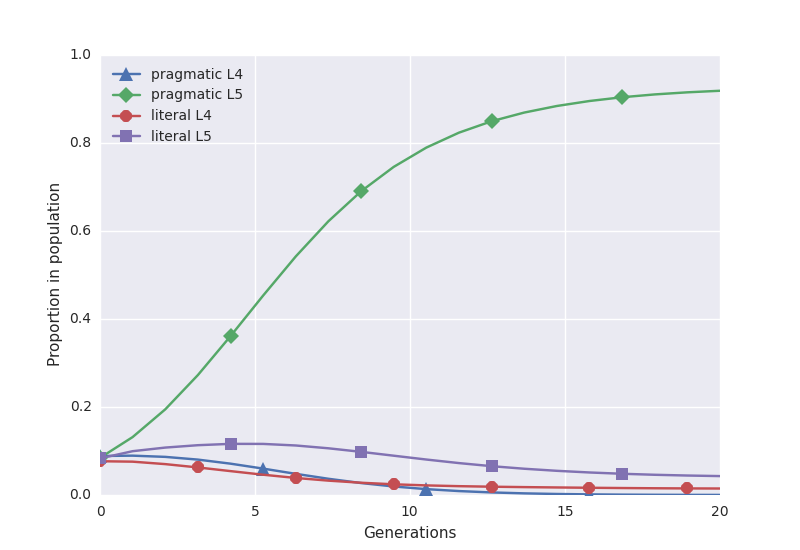
\includegraphics{figure1}}
	\caption{Mean proportions of target types across $20$ generations of $1000$ populations ($\alpha = 1, \lambda = 50, k = 20, c = 0.85$).}
	\label{fig:c-85}
\end{figure}

\begin{figure}[t] %htb for exact position
	\centering
	\resizebox{9.5cm}{!}{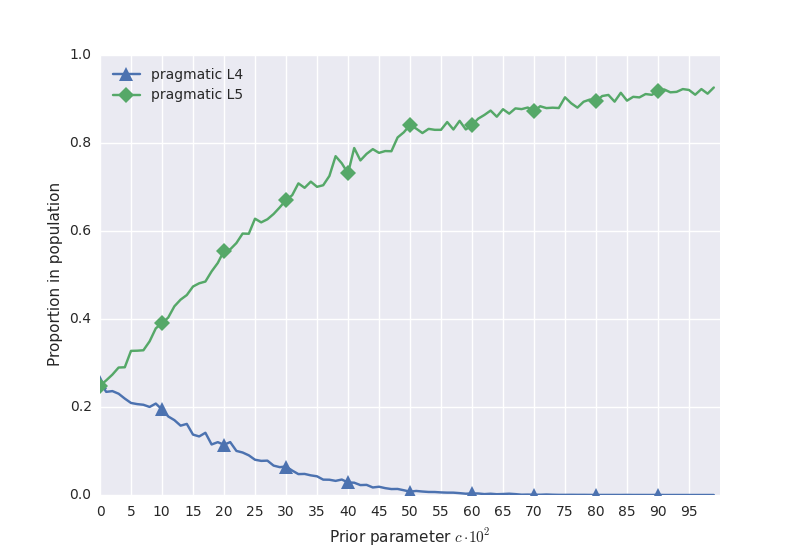
\includegraphics{figure2-cost}}
	\caption{Mean proportion of pragmatic $L_4$ and $L_5$ types after $20$ generations with $c \in [0,1]$ in $1000$ populations ($\alpha = 1, \lambda = 50, k = 20$).}
	\label{fig:cost}
\end{figure}

\begin{table}
\centering 
\begin{tabular}{l c c c c c c c}
~ & 0 & .01 & 0.03 & 0.05 & 0.07 & 0.09 & 0.85\\ \hline \hline
lit. $L_1$& .001 & .002 & .002& .004&.004& .002 & .004\\
lit. $L_2$& .001 & .002 & .001& .001&.001&0& 0\\
lit. $L_3$& .001 & .003 & .001& .002&.002& .001& .004\\
lit. $L_4$& .193 & .193 & .165& .177&.187&.142& .022\\
lit. $L_5$& .022 & .022 & .039& .04&.033&.049& .042\\
lit. $L_6$& .023 & .023 & .028& .027&.028&.025& .002\\ \hline
prag. $L_1$ & .001 & .001 &.001& .002&.004&.003& .005 \\
prag. $L_2$ & .001 & .001 &.001& .001&.001&0 & 0 \\
prag. $L_3$ & .001 & .002 &.002& .002&.004&.002& .006 \\ 
prag. $L_4$ & .257 & .234 &.23& .209&.205&.208& 0 \\
prag. $L_5$ & .249 & .26 & .29& .328& .329& .379& .914 \\
prag. $L_6$ & .25 & .237 & .24& .207& .202&.188& 0 


\end{tabular}
\caption{Mean proportion of types in $1000$ populations after $20$ generations across different bias values $c$ ($\alpha = 1, \lambda = 50, k = 20$).}

\label{tab:numeric-results}
\end{table}

In sum, the results show that in the present setup a weak bias is sufficient to lead to a selection of $L_5$ over $L_4$. This effect increases with the bias' strength provided $L_5$ users are pragmatic. That is, such a learning bias may prevent the lexicalization of pragmatic inferences and explain the prevalence of $L_5$-like semantics. However, note that literal $L_5$ is underrepresented across all values of $c$. This highlights that, while the bias plays a major role for the contrast between $L_4$ and $L_5$, in itself it does not enable types that fail to convey an upper-bound to establish themselves in the population. This suggests pragmatic reasoning to be paramount to the selection of $L_5$-like semantics. That is, neither the learning bias nor functional pressure alone but their combination lead to the systematic lack of semantic upper-bounds in scalar expressions.




\section{Discussion}
Broadly speaking these results confirm our expectations that a lack of semantic upper-bounds coupled with pragmatic reasoning can overcome selective pressures and stabilize in a population provided there is a bias for simpler representations. This outcome is particularly encouraging in light of the potential additional advantages of a lack of semantic upper-bounds discussed above that were not considered here. 

The model gives a justification for lexicalization patterns found in natural language, as well as for the failure to lexicalize certain pragmatic inferences. That is, while the puzzle raised by semantics is hard to explain by purely functional means, we suggest part of the answer to lie in learnability. Simpler semantic representations are more likely to be learned, and pragmatic reasoning can counteract functional disadvantages  otherwise incurred. This result is of particular relevance for the longstanding assumption of a divide and interaction between semantics and pragmatics and offers an account of why (certain) pragmatic inferences are not part of the literal meaning of expressions. It furthermore leaves open the possibility of such inferences to fossilize when they do not compete against a lexical simplicity bias.

A virtue of this model is that it allows for analysis specific modifications and extensions. Straightforward extensions include larger hypothesis spaces, as well as larger or different lexicon fragments. Another worthwhile modification relates to possible disadvantages of pragmatic reasoning. We tacitly assumed pragmatic reasoning to come at no cost. However, there is experimental evidence for the assumption that the pragmatic derivation of upper-bounds costs effort and takes additional processing time (cf. \citealt{deNeys+schaeken:2007, huang+snedeker:2009}). This raises the question at which point such usage-based cost undercuts the learnability advantage of simpler semantic representations.\footnote{In the present setup this modification has a straightforward effect: A penalty for pragmatic signaling lowers the fitness of pragmatic types, to the advantage of literal types. However, the penalty needs to be substantial to counteract the functional advantage pragmatic $L_5$ has over all but $L_4$ together with its learning advantage.}

\begin{figure}[t] %htb for exact position
	\centering
	\resizebox{9.5cm}{!}{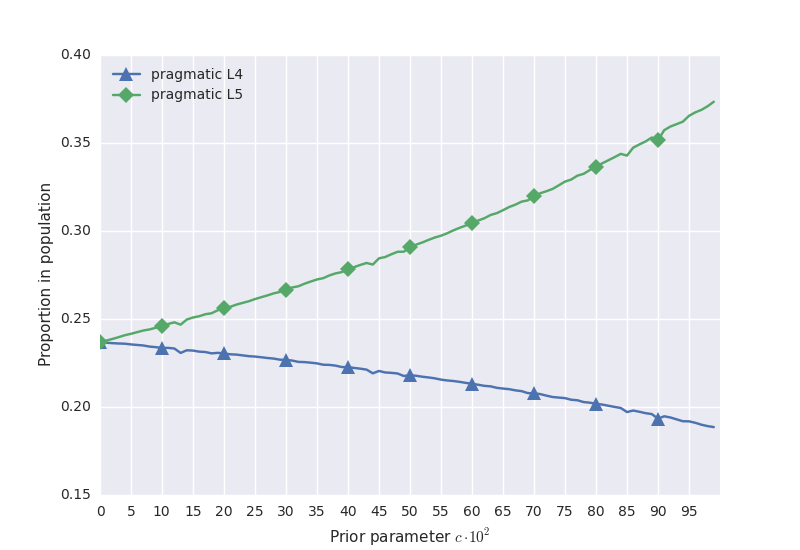
\includegraphics{figure3-parental}}
	\caption{Mean proportion of pragmatic $L_4$ and $L_5$ types after $20$ generations of parental teaching with $c \in [0,1]$ in $1000$ populations ($\alpha = 1, \lambda = 50, k = 20$).}
	\label{fig:figure3-parental}
\end{figure}


Lastly, a crucial component of this model is the learning matrix $Q$ together with its weighted variant $N$. The latter describes ``communal teaching'' where learning a lexicon is influenced by its proportional representation in the preceding generation. This diverges from the mean field dynamics of classical (dynamic) evolutionary game theory and iterated learning. Replacing the weighted matrix $N$ by $Q$, i.e. not weighting the learning matrix, allows for an inspection of the model's predicted outcome for a more classical case of ``parental teaching''. Figure \ref{fig:figure3-parental} shows the effect of the learning bias for this case (cf. Figure \ref{fig:cost}).

Note first that the main result of the prior driving selection of $L_5$ over $L_4$ holds here as well. However, the resulting populations are more heterogeneous than in the communal setting.  The intuition behind communal learning was that learning is influenced by the proportion in which languages are used in a population. However, a stage of exposure to communal language use is currently not represented in the model but only implicit in the weights applied to the Bayesian learning matrix. This step may be regarded as conceptually problematic given that it assumes ``implicit exposure'' to the true distribution of types in the population. Notwithstanding, we see it as a first step in the right direction to capture what constitutes an important factor in learning pressures. Further, it retains but strengthens the results obtained from a more standard learning setup. It is nevertheless important to highlight the weaker results obtained from parental learning as they suggest a missing piece to our overall account. Ideally one would expect the dynamics to favor a well-adapted lexicon over time even when only learning from parents, offering a stronger justification for the advantage of a lexicon without a population's involvement in the learning process. It is possible that a more complex setup where the speaker wants to convey not only bounded but also upper-unbounded states may shed light on this issue, as discussed in \S 2. Alternatively, a similarity bias over lexica may enable for a gradual adoption of particular languages.  A more involved analysis and comparison between static learning matrices and weighted variants, as well as an explicit representation of exposure to linguistic data from the population raise many interesting technical and conceptual challenges we hope to see addressed in the future.






\section{Conclusion}
The development of natural languages is driven by complex intertwined pressures. Drawing from past insights we put forward a model that allows for a general and malleable integration of core aspects involved in this process. Chiefly, the model combines functional pressure, iterated Bayesian learning, and probabilistic speaker and hearer models.  In particular, this analysis addresses longstanding issues concerning the semantics-pragmatics divide. It shows that when pressured for learnability and expressivity, the former force drives for simpler semantic representations inasmuch as pragmatics can compensate for them in language use. Consequently, semantic patterns can be explained in virtue of the linguistic behavior of their users and their complexity. Furthermore, the ease of acquisition of simpler semantics offers an answer to why natural languages do not lexicalize certain pragmatic inferences.





\section{Acknowledgments}
TB acknowledges funding from the European Community's Seventh Framework Programme (FP7/2007-2013) under grant agreement no. 567652 /{\em ESSENCE}/. MF gratefully acknowledges financial support by the Institutional Strategy of the University of T\"ubingen (Deutsche Forschungsgemeinschaft, ZUK 63). RvR acknowledges support by the `Language in Interaction' Gravitation project, funded by NWO.


%\bibliographystyle{unsrtnat}

\bibliographystyle{apacite}

\setlength{\bibleftmargin}{.125in}
\setlength{\bibindent}{-\bibleftmargin}
\bibliography{./cogsci-bib}



\end{document}
